\begin{pastexam}[label={px:ncku-113-prog-04}]{成大資訊聯招 113 學年度 第 4 題}
（單選）

\textbf{[2\%, 3\%]} Given the following weighted undirected graph.
\begin{center}
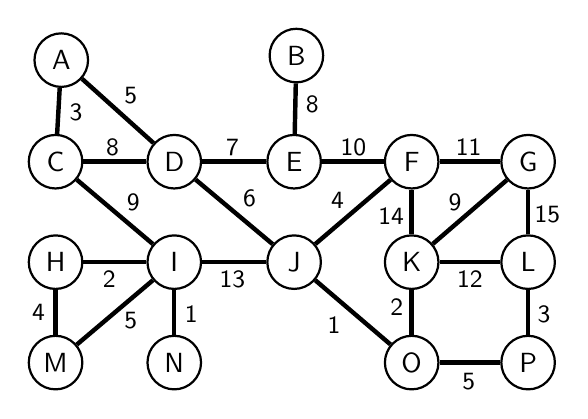
\begin{tikzpicture}[x=0.0145cm,y=-0.0145cm,v/.style={circle,draw,thick,fill=white,inner sep=0pt,minimum size=0.68cm,font=\sffamily},w/.style={font=\sffamily\small,inner sep=0pt}]
\node[v] (A) at (461,291) {A};
\node[v] (B) at (667,287) {B};
\node[v] (C) at (456,380) {C};
\node[v] (D) at (560,380) {D};
\node[v] (E) at (665,380) {E};
\node[v] (F) at (768,380) {F};
\node[v] (G) at (870,380) {G};
\node[v] (H) at (456,468) {H};
\node[v] (I) at (560,468) {I};
\node[v] (J) at (665,468) {J};
\node[v] (K) at (768,468) {K};
\node[v] (L) at (870,468) {L};
\node[v] (M) at (456,556) {M};
\node[v] (N) at (560,556) {N};
\node[v] (O) at (768,556) {O};
\node[v] (P) at (870,556) {P};
\draw[line width=1.6pt] (A)--(C);
\node[w] at (474,337) {3};
\draw[line width=1.6pt] (A)--(D);
\node[w] at (522,322) {5};
\draw[line width=1.6pt] (C)--(D);
\node[w] at (506,367) {8};
\draw[line width=1.6pt] (C)--(I);
\node[w] at (524,416) {9};
\draw[line width=1.6pt] (D)--(E);
\node[w] at (611,367) {7};
\draw[line width=1.6pt] (D)--(J);
\node[w] at (626,412) {6};
\draw[line width=1.6pt] (B)--(E);
\node[w] at (681,330) {8};
\draw[line width=1.6pt] (E)--(F);
\node[w] at (717,367) {10};
\draw[line width=1.6pt] (F)--(J);
\node[w] at (703,414) {4};
\draw[line width=1.6pt] (F)--(K);
\node[w] at (750,428) {14};
\draw[line width=1.6pt] (F)--(G);
\node[w] at (818,367) {11};
\draw[line width=1.6pt] (G)--(K);
\node[w] at (806,416) {9};
\draw[line width=1.6pt] (G)--(L);
\node[w] at (887,426) {15};
\draw[line width=1.6pt] (K)--(L);
\node[w] at (819,483) {12};
\draw[line width=1.6pt] (H)--(I);
\node[w] at (503,483) {2};
\draw[line width=1.6pt] (H)--(M);
\node[w] at (441,512) {4};
\draw[line width=1.6pt] (I)--(M);
\node[w] at (522,519) {5};
\draw[line width=1.6pt] (I)--(N);
\node[w] at (575,514) {1};
\draw[line width=1.6pt] (I)--(J);
\node[w] at (611,483) {13};
\draw[line width=1.6pt] (J)--(O);
\node[w] at (700,523) {1};
\draw[line width=1.6pt] (K)--(O);
\node[w] at (755,508) {2};
\draw[line width=1.6pt] (L)--(P);
\node[w] at (884,514) {3};
\draw[line width=1.6pt] (O)--(P);
\node[w] at (818,572) {5};
\end{tikzpicture}
\end{center}

\begin{enumerate}[label=\roman*)]
\item Which of the following statements is correct?
\begin{enumerate}[label=(\Alph*)]
\item When performing a depth first search of this graph, the next node to visit can be D after
visiting A, C, I, N, M, and H.
\item When performing a breath first search of this graph, the next node to visit can be D after
visiting A, C, I, N, M, and H.
\item When performing a depth first search of this graph, the next node to visit can be K after
visiting B, E, and F.
\item When performing a breath first search of this graph, the next node to visit can be K after
visiting B, E, and F.
\item None of the above
\end{enumerate}
\item After generating a \underline{maximum} cost spanning tree from this graph, which of the
following statements is correct?
\begin{enumerate}[label=(\Alph*)]
\item The degree of the node F in the resultant maximum cost spanning tree is 3.
\item The cost of the resultant maximum cost spanning tree is 118.
\item (O, P) is an edge of the resultant maximum cost spanning tree.
\item In the resultant maximum cost spanning tree, the number of edges on the path from A to O is
6.
\item None of the above
\end{enumerate}
\end{enumerate}
\end{pastexam}

\begin{pastsoln}
答案：i) (C)；ii) (C)。 i) 是 DFS、BFS（資結書第~21~章），ii) 是生成樹（第~24~章），配分 ii) 比較
重，所以放在第~24~章。 原題的「breath first」是「breadth first」的筆誤。

先列出每個頂點的鄰居：A: C, D；B: E；C: A, D, I；D: A, C, E, J；E: B, D, F；F: E, G, J, K；
G: F, K, L；H: I, M；I: C, H, J, M, N；J: D, F, I, O；K: F, G, L, O；L: G, K, P；M: H, I；N: I；
O: J, K, P；P: L, O。 題目沒有規定鄰居的順序，所以「can be」是問：有沒有某一種鄰居順序讓它發生。

\textbf{i)}
\begin{itemize}
\item (A) 錯。 DFS 的順序 A, C, I, N, M, H 本身做得到：A $\to$ C $\to$ I $\to$ N（N 只有 I 一個鄰居，退回 I）
$\to$ M $\to$ H。 H 的鄰居 I、M 都拜訪過，退回 M；M 的鄰居也都拜訪過，退回 I。 這時 I 還有一個
沒拜訪的鄰居 J，DFS 一定先走 J，不會退回 C 去走 D。 下一個只能是 J。
\item (B) 錯。 BFS 從 A 開始，先拜訪 A 的所有鄰居 C、D，才輪到第二層的頂點。 I 離 A 的距離是 $2$，
D 是 $1$，D 一定比 I 先被拜訪，「A, C, I」這個開頭不可能出現在 BFS 裡。
\item (C) 對。 DFS 從 B 開始，B $\to$ E（唯一的鄰居）$\to$ F（E 的鄰居可以先選 F）$\to$ K（F 的鄰居可以
先選 K）。 只要鄰居的順序讓 E 先走 F、F 先走 K 就行。
\item (D) 錯。 BFS 從 B 開始：B，再來是 E，再來是 E 的鄰居 D、F（順序可以換）。 拜訪完 B, E, F 之後，
佇列裡還有 D，它和 F 同一層，一定比 F 的鄰居 K 先被拜訪，下一個只能是 D。
\end{itemize}

\textbf{ii)} 最大生成樹：把 Kruskal 演算法（資結書虛擬碼~24.2）的邊改成由大到小排序，不形成環就
選（理由見資結書第~24.2~節：權重全部取負號，最小生成樹就是原圖的最大生成樹）。 圖有 $16$ 個頂點，
要選 $15$ 條邊。
\begin{center}
\small
\begin{tabular}{clcl}
\toprule
權重 & 邊與結果 & 權重 & 邊與結果 \\
\midrule
15 & (G, L) 選 & 6 & (D, J) 不選：D--C--I--J 已連通 \\
14 & (F, K) 選 & 5 & (A, D) 選 \\
13 & (I, J) 選 & 5 & (I, M) 選 \\
12 & (K, L) 選 & 5 & (O, P) 選 \\
11 & (F, G) 不選：F--K--L--G 已連通 & 4 & (F, J) 不選：F--E--D--C--I--J 已連通 \\
10 & (E, F) 選 & 4 & (H, M) 選 \\
9 & (C, I) 選 & 3 & (A, C) 不選：A--D--C 已連通 \\
9 & (G, K) 不選：G--L--K 已連通 & 3 & (L, P) 選 \\
8 & (C, D) 選 & 2 & (H, I) 不選：H--M--I 已連通 \\
8 & (B, E) 選 & 2 & (K, O) 不選：K--L--P--O 已連通 \\
7 & (D, E) 選 & 1 & (I, N) 選 \\
 & & 1 & (J, O) 不選：已連通 \\
\bottomrule
\end{tabular}
\end{center}
選了 $15$ 條：(G,L), (F,K), (I,J), (K,L), (E,F), (C,I), (C,D), (B,E), (D,E), (A,D), (I,M), (O,P),
(H,M), (L,P), (I,N)，總權重
\[
15 + 14 + 13 + 12 + 10 + 9 + 8 + 8 + 7 + 5 + 5 + 5 + 4 + 3 + 1 = 119 .
\]
圖裡有相同權重的邊，但每一條沒選的邊，都比它和樹上路徑形成的環上其他邊都輕（例如 (F, G) 的 $11$
小於 F--K--L--G 上的 $14, 12, 15$），由環性質（資結書定理~24.3，把「最重」換成「最輕」），它不在任何一棵
最大生成樹裡，所以最大生成樹是唯一的，下面的判斷不受同權重的影響。
\begin{itemize}
\item (A) 錯。 樹裡和 F 相連的邊只有 (F, K)、(E, F)，度數是 $2$。
\item (B) 錯。 總成本是 $119$，不是 $118$。
\item (C) 對。 (O, P) 的權重 $5$ 被選進樹。
\item (D) 錯。 樹上 A 到 O 的路徑是 A--D--E--F--K--L--P--O，共 $7$ 條邊。
\end{itemize}
\end{pastsoln}
